%arara: lualatex: { branch: developer, interaction: errorstopmode,
%arara: --> shell: yes, synctex: yes }
%arara: makeglossaries if found('aux', '@istfilename')
%arara: biber: { options: [ '--wraplines' ] }

\documentclass[%
% aspectratio=169,
spanish,
mexico]{beamer}
\mode<presentation>

\usepackage{babel}

\usetheme[progressbar=foot]{metropolis}
% \usecolortheme{seahorse}
% \usetheme{Warsaw}
% \usecolortheme{albatross}

\setbeamercolor{figure}{fg==black!2,bg=mDarkTeal}

\usepackage{fontspec}
    \setmainfont{TeX Gyre Pagella}
    \setsansfont{TeX Gyre Heros}

\renewcommand{\familydefault}{\sfdefault} % Sans serif

\usepackage{csquotes}
\MakeAutoQuote{“}{”}

\usepackage{microtype}
\setlength{\parskip}{1em}
\usepackage{tabularray}
    \UseTblrLibrary{booktabs}
    \UseTblrLibrary{siunitx}
    \DefTblrTemplate{contfoot-text}{normal}{\itshape Continúa en la siguiente página}
    \SetTblrTemplate{contfoot-text}{normal}
    \DefTblrTemplate{conthead-text}{normal}{\itshape (Continuación)}
    \SetTblrTemplate{conthead-text}{normal}

\usepackage{siunitx}
\sisetup{separate-uncertainty,per-mode=symbol,detect-all}
\DeclareSIUnit{\angstrom}{\textup{\AA}}

\usepackage{glossaries}
    \makeglossaries{}

\usepackage[style=alphabetic,backend=biber,url=false]{biblatex}
    \addbibresource[location=remote]{http://127.0.0.1:23119/better-bibtex/export/library?/1/library.biblatex}

	\setbeamerfont{footnote}{size=\tiny}
	\renewcommand{\footnotesize}{\tiny}
	\AtEveryCitekey{\iffootnote{\color{red}\tiny}{\color{blue}}}
	

\usepackage[skins]{tcolorbox}
\usepackage{paralist}
\usepackage{cleveref}
\usepackage{subcaption}
\usepackage[colorinlistoftodos]{todonotes}
\usepackage{lineno}
\usepackage{rotating}
\usepackage{newfloat}
\usepackage{float}
\DeclareFloatingEnvironment[
   fileext=los,
   listname={List of Schemes},
   name=Scheme,
   placement=tbp,
   within=none % don't reset numbering
]{scheme}
\DeclareCaptionSubType{scheme}
\setcounter{secnumdepth}{5}

\begin{filecontents}[force]{abreviaturas.tex}
    \newacronym{DFT}{DFT}{Teoría del funcional de la densidad \textit{(del inglés ``Density Functional Theory'')}}
    \newacronym{TDDFT}{TDDFT}{Teoría del funcional de la densidad tiempo-dependiente \textit{(del inglés ``Time-Dependant Density Functional Theory'')}}
    \newacronym{FMR}{FMR}{Rotores Moleculares Fluorescentes \textit{(Del inglés ``Flurescent Molecular Rotor'')}}
    \newacronym{BOSCHIBA}{BOSCHIBA}{Bases de Schiff de Boro \textit{(del inglés ``\textsc{Bo}ron \textsc{Schi}ff \textsc{Ba}ses'')}}
    \newacronym{BODIPY}{BODIPY}{\textsc{bo}ron-\textsc{di}\textsc{py}rromethene}
    \newacronym{TICT}{TICT}{transferencia de carga intramolecular retorcida \textit{(del inglés ``twsited intramolecular charge transfer'')}}
    \newacronym{LE}{LE}{Local Excitado \textit{(del inglés ``locally exited'')}}
    \newacronym{MW}{MW}{Microondas \textit{(del inglés ``Microwave'')}}
    \newacronym{PES}{PES}{Superficie de Energía Potencial \textit{(del inglés ``Potential Energy Surface'')}}
    \newacronym{NBO}{NBO}{Orbitales Naturales de Enlace \textit{(del inglés ``Natural Bond Orbitals'')}}
    \newacronym{ICT}{ICT}{Transferencia de Carga Intramolecular \textit{(del inglés ``Intramolecular Charge Transfer'')}}
    \newacronym{VEE}{VEE}{Energía de Emisión Vertical \textit{(del inglés ``Vertical Emission Energy'')}}
    \newacronym{FMO}{FMO}{Orbitales Moleculares de Frontera \textit{(del inglés ``Frontier Molecular Orbitals'')}}
    \newacronym{HOMO}{HOMO}{Orbital Molecular de mas alta energía \textit{(del inglés ``Highest Occupied Molecular Orbital'')}}
    \newacronym{LUMO}{LUMO}{Orbital Molecular no ocupado de más baja energía \textit{(del inglés ``Lowest Unoccupied Molecular Orbital'')}}
    \newacronym{NMR}{NMR}{Resonancia Magnética Nuclear \textit{(del inglés ``Nuclear Magnetic Resonance'')}}
    \newacronym{CREST}{CREST}{\textit{Conformer-Rotamer Ensemble Sampling Tool}}
\end{filecontents}

\begin{filecontents}[force]{comandos.tex}
    % \newcommand{\invitro}{\textit{in-vitro}}
    \newcommand\scan{\(\text{r}^{2}\text{SCAN-3c}\)}
    
\end{filecontents}

\begin{filecontents}[force]{quimica.tex}
    \usepackage{chemmacros}
    \DeclareChemReactant{BO-gly}{name={BO-Gly}} % 1
    \DeclareChemReactant{BO-trp}{name={BO-Trp}} % 2
    \DeclareChemReactant{BO-tyr}{name={Bo-Tyr}} % 3
    \DeclareChemReactant{BO-phe}{name={BO-Phe}} % 4
    \DeclareChemReactant{trp}{name={\iupac{\laevus-triptófano}}, short={trp}}
    \DeclareChemReactant{phe}{name={\iupac{\laevus-fenilalanina}}, short={phe}}
    \DeclareChemReactant{tyr}{name={\iupac{\laevus-tirosina}}, short={tyr}}
    \DeclareChemReactant{gly}{name={glicina}, short={gly}}
    \DeclareChemReactant{aphb}{name={ácido fenil borinico}, short={\ch{PhB(OH)2}}}
    \DeclareChemReactant{2h1n}{name={\iupac{2-Hidroxi-1-naftaldehido}}, short={\iupac{2-Hidroxi-1-naftaldehido}}}
    \NewChemLatin\invitro{in vitro}
    \NewChemLatin\invivo{in vivo}
    \NewChemLatin\insilico{in silico}
    \DeclareChemTranslation{scheme-name}{spanish}{Esquema}
    \DeclareChemTranslation{scheme-list}{spanish}{Lista de esquemas}
    \DeclareChemTranslation{scheme}{spanish}{esquema}
    \DeclareChemTranslation{schemes}{spanish}{esquemas}
    \DeclareChemTranslation{Scheme}{spanish}{Esquema}
    \DeclareChemTranslation{Schemes}{spanish}{Esquemas}
    \chemsetup{language=spanish}
    % \renewcommand{\schemename}{Esquema}
    % \AtBeginDocument{
    % \renewcommand{\tablename}{Tabla}
    % }
    
    \AtBeginDocument{%
    \addto\captionsspanish{\renewcommand\listschemename{Índice de esquemas}}%
    \addto\captionsspanish{\renewcommand\schemename{Esquema}}%
    \csname captions\languagename\endcsname
}
    % \chemsetup[reactants]{printreactants-style=xltabular}
\end{filecontents}

%% LaTeX2e file `abreviaturas.tex'
%% generated by the `filecontents' environment
%% from source `PEAG-Protocolo_maestria' on 2023/09/17.
%%
    \newacronym{DFT}{DFT}{Teoría del funcional de la densidad \textit{(del inglés "Density Functional Theory")}}
    \newacronym{TDDFT}{TDDFT}{Teoría del funcional de la densidad tiempo-dependiente \textit{(del inglés "Time-Dependant Density Functional Theory")}}
    \newacronym{FMR}{FMR}{Rotores Moleculares Fluorescentes \textit{(Del inglés Flurescent Molecular Rotor)}}
    \newacronym{BOSCHIBA}{BOSCHIBA}{Bases de Schiff de Boro \textit{(del inglés "\textsc{Bo}ron \textsc{Schi}ff \textsc{Ba}ses")}}
    \newacronym{BODIPY}{BODIPY}{\textsc{bo}ron-\textsc{di}\textsc{py}rromethene}
    \newacronym{TICT}{TICT}{transferencia de carga intramolecular retorcida \textit{(del inglés "twsited intramolecular charge transfer")}}
    \newacronym{LE}{LE}{local excitado \textit{(del inglés "locally exited")}}

%% LaTeX2e file `comandos.tex'
%% generated by the `filecontents' environment
%% from source `Presentación-Protocolo-Maestria-PEAG' on 2023/11/14.
%%
    % \newcommand{\invitro}{\textit{in-vitro}}
    \newcommand\scan{\(\text{r}^{2}\text{SCAN-3c}\)}


%% LaTeX2e file `quimica.tex'
%% generated by the `filecontents' environment
%% from source `PEAG-Protocolo_maestria' on 2023/09/17.
%%
    \DeclareChemReactant{BO1}{name={BO1}, short={THF}}
    \DeclareChemReactant{BO-trp}{name={triptófano}, short={BO-trp}}
    \DeclareChemReactant{BO-phe}{name={fenilalanina}, short={BO-phe}}
    \DeclareChemReactant{BO-tyr}{name={tirosina}, short={BO-tyr}}
    \DeclareChemReactant{BO-gly}{name={glicina}, short={BO-gly}}
    \NewChemLatin\invitro{in vitro}
    \NewChemLatin\insilico{in silico}
    \DeclareChemTranslation{scheme-name}{spanish}{Esquema}
    \DeclareChemTranslation{scheme-list}{spanish}{Lista de esquemas}
    \DeclareChemTranslation{scheme}{spanish}{esquema}
    \DeclareChemTranslation{schemes}{spanish}{esquemas}
    \DeclareChemTranslation{Scheme}{spanish}{Esquema}
    \DeclareChemTranslation{Schemes}{spanish}{Esquemas}
    \renewcommand{\schemename}{Esquema}


% \renewcommand{\iffootnote}{\scriptsize}

\title{Síntesis sustentable, caracterización química-fotofísica, y por DFT de BOSCHIBA derivadas de aminoácidos y su aplicación \invitro{}}
\subtitle{Protocolo de tesis de maestría}
\date{2023--11--30}
\author{Pablo E. Alanis}
\institute{Universidad Autónoma de Nuevo León, División de Posgrado}

\begin{document}
\maketitle

\begin{frame}{Contenido}
	\tableofcontents
\end{frame}

% \begin{frame}
%     \begin{itemize}[<+- | alert@+>]
%         \item Se evaluó con \fbox{FabH} y \fbox{FabI}
%         \item Se determinó la afinidiad en los sitios activos de estas proteínas
%         \item Se usó SYBYL-X 2.0 para determinar la afinidad $K_b$
%     \end{itemize}
% \end{frame}

\section{Resumen}

\begin{frame}[standout]
	\small
	\vspace*{\fill}
	Se sintetizarán una serie de \gls{BOSCHIBA} derivadas de \reactant*{gly}, \reactant*{trp}, \reactant*{tyr} y \reactant*{phe}. Se caracterizarán por métodos espectroscópicos y se realizarán cálculos \insilico{} por medio de \gls{DFT} y \gls{TDDFT} para estudiar las propiedades fotofísicas de los compuestos y comprobar los mecanismos involucrados en el efecto supresor de la luminiscencia en dichos compuestos así como estudios de topológicos sobre los mismos. A su vez, se realizarán estudios de citotoxicidad y tinción \invitro{} para determinar su actividad biológica de los compuestos.
	\vspace*{\fill}
\end{frame}

\section{Introducción}
\begin{frame}{Introducción}
	\begin{itemize}
		\item Interés en compuestos fluorescentes de boro;
		\item Amplio campo de aplicaciones;
		\item BODIPY comercialmente disponibles;
		      \begin{itemize}
			      \item Utilizados como agentes para la tinción celular:
			            \begin{enumerate}
				            \item ER-Tracker™ Green, y;
				            \item ER-Tracker™ Red.
			            \end{enumerate}
		      \end{itemize}
	\end{itemize}
\end{frame}

{
\setbeamercolor{background canvas}{fg=black!2, bg=white}
\begin{frame}{ER-Tracker™}
	\begin{scheme}[H]
		\centering
		\begin{subscheme}{0.45\linewidth}
			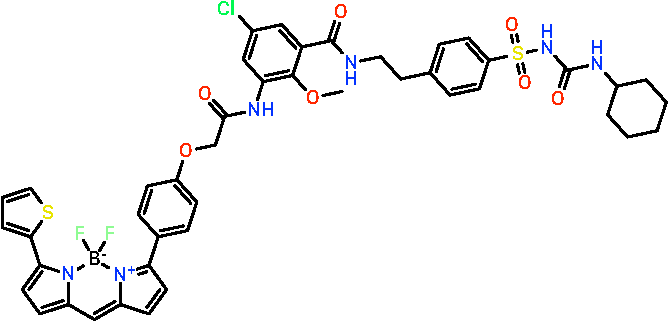
\includegraphics[width=\linewidth]{./Figuras/ER-Tracker_Blue.pdf}
			\caption{ER-Tracker™ Blue}
			\label{ER-Tracker_Blue}
		\end{subscheme}
		\hfill
		\begin{subscheme}{0.45\linewidth}
			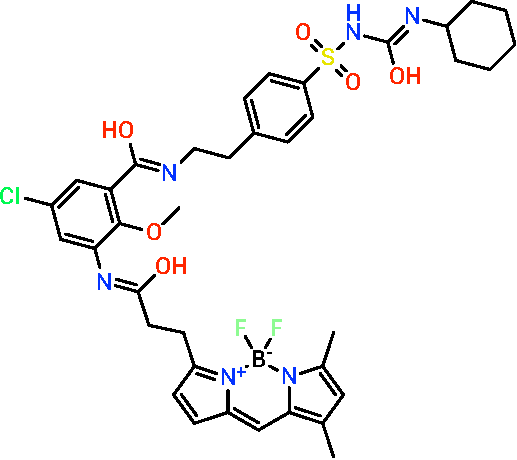
\includegraphics[width=\linewidth]{./Figuras/ER-Tracker_Green.pdf}
			\caption{ER-Tracker™ Green}
			\label{ER-Tracker_Green}
		\end{subscheme}
		\caption[ER-Trackers™]{\textit{Los ER-Tracker™ Green} y \textit{ER-Tracker™ Red} de Thermo Fischer Scientific™ son \gls{BODIPY} comerciales utilizados como agentes para la tinción celular.}
		\label{ER-Trackers}
	\end{scheme}
\end{frame}
}


\begin{frame}{Fluoróforos sensibles a la viscosidad i}
	\begin{itemize}
		\item Los \gls{FMR} son fluoróforos sensibles a la viscosidad.
		\item Presentan una rotación libre que se vuelven fluorescentes.
		\item Aumentan la fluorescencia solo si su rotación se ve restringida.
	\end{itemize}
\end{frame}
\setbeamerfont{footnote}{size=\tiny}
\begin{frame}{Fluoróforos sensibles a la viscosidad ii}
	\begin{itemize}
		\item Algunas interacciones de carácter intramolecular para detener la rotación de los \gls{FMR} son:
		      \begin{enumerate}[i.]
			      \item Formar interacciones de hidrógeno;\footcite{wuMultistageRotationalSpeed2018}
			      \item A través del impedimento estérico;\footcite{faulknerAllostericRegulationRotational2016} o
			      \item Por la formación de complejos estables con iones metálicos.\footcite{yadavViscochromicMechanochromicUnsymmetrical2019}
		      \end{enumerate}
	\end{itemize}
\end{frame}

\begin{frame}{Fluoróforos sensibles a la viscosidad iii}
	\begin{itemize}
		\item Se ha determinado que la polaridad del solvente y la viscosidad del mismo afectan considerablemente la fluorescencia de los \gls{FMR}.
		\item El efecto que tiene la polaridad del solvente, aunque se sabe que es importante, no se ha logrado elucidar de forma aislada a la viscosidad.\footfullcite{haidekkerEffectsSolventPolarity2005}
	\end{itemize}
\end{frame}

\begin{frame}[allowframebreaks]{Referencias}
	\small
	\printbibliography{}
\end{frame}

\begin{frame}[allowframebreaks]{Glosario}
	\small
	% \printglossaries[nonumberlist]{}
	\printglossary[type=main,style=long,nonumberlist]
\end{frame}

\end{document}
